\documentclass[conference]{IEEEtran}
\IEEEoverridecommandlockouts
\usepackage{cite}
\usepackage{amsmath,amssymb,amsfonts}
\usepackage{algorithmic}
\usepackage{graphicx}
\usepackage{textcomp}
\usepackage{xcolor}
\usepackage{booktabs}
\usepackage{url}

\graphicspath{{figures/}}

\def\BibTeX{{\rm B\kern-.05em{\sc i\kern-.025em b}\kern-.08em
    T\kern-.1667em\lower.7ex\hbox{E}\kern-.125emX}}

\begin{document}

\title{Learn To Tag --- A Reinforcement Learning Environment with\\
Multi-Algorithm Agent Comparison and Human-in-the-Loop Training}

\author{%
\IEEEauthorblockN{1\textsuperscript{st} Ghanibhuti Gogoi}
\IEEEauthorblockA{\textit{HKUST GZ} \\
Student ID: 50014104 \\
ggogoi543@connect.hkust-gz.edu.cn}
\and
\IEEEauthorblockN{2\textsuperscript{nd} Siqi Chen}
\IEEEauthorblockA{\textit{HKUST GZ} \\
Student ID: 50012493 \\
schen@connect.hkust-gz.edu.cn}
\and
\IEEEauthorblockN{3\textsuperscript{rd} Yuhan Chen}
\IEEEauthorblockA{\textit{HKUST GZ} \\
Student ID: 50013198 \\
ychen590@connect.hkust-gz.edu.cn}
}

\maketitle

\begin{abstract}
We present \textit{Learn To Tag}, a multi-agent Tag environment as a
controlled testbed for benchmarking reinforcement learning (RL) algorithms
under \emph{mid-episode role switching}. In our environment, six agents move
continuously through a 2D grid; one is the ``tagger'' and the rest are
runners. When a tagger reaches a runner the runner becomes the new tagger,
instantaneously inverting that agent's reward signal from chase to flee.
We implement Q-Learning, SARSA, DQN, and PPO under a unified interface, with
all agents sharing two role-specialized networks (a \emph{tagger brain} and a
\emph{runner brain}) selected at runtime by the agent's current role. We
design a minimal pure-proximity reward function with symmetric tagger and
runner shaping, and a unified training and evaluation pipeline that performs
joint evaluation, isolated role evaluation against a random opponent, and
behavioral visualization. The environment also supports a human-in-the-loop
mode in which a human player competes against agents that continue to learn
in real time. Our results show that tabular methods fail to learn on the
full continuous environment (zero successful tags across 1000 epochs) but
converge cleanly on a simplified $10{\times}10$ turn-based gridworld
variant. DQN learns a competitive joint policy, achieving an isolated
tagger score of 41.85 tags per 2000-step evaluation episode at epoch 1000,
and a best-checkpoint joint score of 10.7 tags. The dual-role architecture
and isolated role evaluation expose a consistent asymmetry: tagger policies
saturate quickly while runner policies remain weak, motivating role-aware
algorithm selection and reward shaping in mixed-role multi-agent tasks.
\end{abstract}

\begin{IEEEkeywords}
reinforcement learning, multi-agent systems, pursuit-evasion, role-switching,
deep Q-network, proximal policy optimization, reward shaping,
human-in-the-loop training
\end{IEEEkeywords}

\section{Introduction}

Reinforcement learning (RL) has produced notable successes in cooperative and
competitive multi-agent settings such as Atari, Go, StarCraft, and
hide-and-seek. In nearly all of these benchmarks each agent's role is fixed
for the entire episode---a player is permanently a predator, a defender, or a
forager. The classical playground game of \emph{Tag} is structurally
different. When the tagger touches a runner, the runner instantaneously
\emph{becomes} the new tagger. The same agent must therefore maintain two
opposite policies---a chase policy and a flee policy---and switch between
them mid-episode, conditioned only on a single role flag.

This role-switching property creates a concrete experimental question:
\emph{how do different RL algorithms cope with abrupt mid-episode reward
inversion in a multi-agent setting?} Standard algorithms make different
theoretical assumptions about exploration and risk (off-policy vs.\ on-policy,
value-based vs.\ policy-gradient), and Tag isolates these differences in an
interpretable, visualizable environment.

\textbf{Contributions.} We address this question with three contributions:
\begin{enumerate}
    \item A 2D multi-agent Tag environment in Python/Pygame with a unified
    \texttt{BaseRLAlgorithm} interface, so any new algorithm can be plugged in
    by implementing five methods.
    \item A \emph{dual-role} algorithm wrapper that automatically routes
    observations to a tagger network or a runner network based on the agent's
    current role flag, eliminating the conflicting-gradient problem that
    arises when one network is trained on opposing reward signals.
    \item A unified training and evaluation pipeline that evaluates each
    checkpoint under three protocols---joint evaluation, isolated tagger
    evaluation (trained tagger vs.\ random runners), and isolated runner
    evaluation (trained runners vs.\ random tagger)---and produces matching
    rendered videos so that emergent strategies can be qualitatively
    recognized.
\end{enumerate}

The remainder of this paper is organized as follows.
Section~\ref{sec:problem} formalizes the problem and surveys related work.
Section~\ref{sec:methodology} describes the environment, observation, reward
design, dual-role architecture, and the four implemented algorithms.
Section~\ref{sec:results} reports experimental results and behavioral
analysis. Section~\ref{sec:conclusion} concludes and outlines future work.

\section{Problem Definition and Literature Review}\label{sec:problem}

\subsection{Problem Definition}

We formalize multi-agent Tag as a partially observable stochastic game with
$N=6$ agents. At each time step every agent $i$ observes an ego-centric vector
$o_i \in \mathbb{R}^{43}$ that includes its own position and velocity, the
relative offsets and distances to all other agents, eight wall-raycast
distances, and a binary role flag $b_i \in \{0,1\}$ indicating whether agent
$i$ is currently the tagger. Each agent selects an action
$a_i \in \mathcal{A} = \{\text{stay, up, down, left, right}\}$. A tag event
occurs when the tagger comes within \texttt{TAG\_RADIUS} pixels of any runner;
on such an event the runner respawns at a random spawn point and the role
flag $b$ flips for both involved agents. Reward functions $r_i^{\text{tag}}$
and $r_i^{\text{run}}$ are role-conditional and inverted on every tag, so the
\emph{same} agent receives opposite reward signals at adjacent timesteps.
The objective is to learn role-conditional policies that perform well in both
roles \emph{simultaneously}.

\textbf{Significance.} Role-switching tasks are common in real-world settings
that academic benchmarks rarely capture: traffic intersections (vehicles
alternate between yielding and asserting right-of-way), warehouse robotics
(robots alternate between carrier and obstacle roles), and team sports
(players alternate offense and defense). Tag is the simplest concrete
instance of this class. Solving it cleanly requires (i) a network or
mechanism that does not catastrophically forget the previous role's policy
when the role flips, and (ii) an evaluation protocol that can detect
role-specific failure modes (e.g., a strong tagger but a weak runner) which
joint scoring would hide.

\textbf{Research gap.} Most multi-agent RL benchmarks fix each agent's role
for the entire episode. We are not aware of a published benchmark that
(a) compares tabular and deep RL on the same role-switching task, and
(b) evaluates each role independently with a controlled-opponent protocol.
The present work fills that gap.

\subsection{Literature Review}

\textbf{Tabular methods.} Q-Learning~\cite{watkins1989} and
SARSA~\cite{rummery1994} are the canonical model-free temporal-difference
methods. Q-Learning is off-policy: it bootstraps from
$\max_{a'} Q(s', a')$, ignoring the action actually taken next. SARSA is
on-policy: it bootstraps from the actual next action, which includes
$\epsilon$-random exploration. The two algorithms produce different risk
profiles, classically demonstrated in the Cliff-Walking example
of~\cite{sutton2018}: Q-Learning learns an aggressive optimal path along the
cliff edge, while SARSA learns a safer detour because it accounts for the
chance of falling during exploration. We test whether this risk asymmetry
manifests as role-specialization in a multi-agent pursuit-evasion setting.

\textbf{Deep value-based RL.} DQN~\cite{mnih2015} approximates the
action-value function with a neural network and stabilizes training with
experience replay (decorrelating samples) and a periodically updated target
network (stabilizing the bootstrapping target). Subsequent
extensions~\cite{vanhasselt2016} address overestimation bias, but for the
present comparison we use the original DQN formulation.

\textbf{Deep policy-gradient RL.} PPO~\cite{schulman2017} optimizes a clipped
surrogate objective to enable stable on-policy updates without trust-region
constraints. PPO has become the de-facto standard for cooperative multi-agent
simulation~\cite{yu2022}.

\textbf{Multi-agent pursuit-evasion.} OpenAI's Hide-and-Seek~\cite{baker2020}
demonstrated emergent tool-use in a similar setting using PPO with self-play,
but their environment fixes roles per episode (hider or seeker for the entire
episode), avoiding the mid-episode role inversion that defines our task.

\textbf{Role-conditional and modular policies.} Goal-conditional
RL~\cite{schaul2015} and modular policy
networks~\cite{andreas2017} are conceptually related to our dual-role
wrapper, in that all share the idea of conditioning behavior on a discrete
context flag. Our contribution is the empirical demonstration that this
mechanism solves the conflicting-gradient problem in a continuous-state
multi-agent setting and additionally enables \emph{algorithm} mixing across
roles (Section~\ref{sec:results-discussion}).

\textbf{Difference from prior work.} We compare four algorithms across three
method families on the \emph{same} environment with role-switching dynamics,
and we additionally evaluate each role independently---a protocol that, as
shown in Section~\ref{sec:results}, is essential for diagnosing role-specific
failure modes that joint evaluation hides.

\section{Methodology}\label{sec:methodology}

\subsection{Environment}

The Tag game is implemented as a 2D tile-based world built on Pygame. The
default map (\texttt{level\_small.txt}) is a $16\times 11$ grid
($512\times 352$~pixels at \texttt{TILE\_SIZE}=32) containing six spawn
points, four crate spawns, and a single connected interior region with three
doorways that encourage navigation around obstacles. Six agents are spawned
at random spawn points each round; at any instant one is the tagger and five
are runners. When the tagger collides with a runner, the runner is teleported
to a randomly chosen spawn point and immediately becomes the new tagger.
The game runs at 60~FPS in rendered mode and at unbounded speed in headless
mode for training. Crates are pushable by entities and act as movable cover.

\subsection{Action Space}

Every agent shares the same discrete action space of size 5: \emph{no-op,
up, down, left, right}. Diagonal movement emerges from alternating actions
between decision frames. Decisions are made every
\texttt{DECISION\_INTERVAL}=2 frames, so an agent acts at 30~Hz; rewards
accumulated between decisions are summed into a single learning signal per
decision step.

\subsection{Observation}\label{sec:obs}

We use a fixed-size 43-dimensional ego-centric observation vector
(Fig.~\ref{fig:observation}, Table~\ref{tab:obs}). Every position is
normalized either to $[0, 1]$ in
the global frame or by the map's diagonal length when expressed as a
relative offset. Eliminated agents are filtered out so that policies do
not perceive or act upon inactive opponents. To give the policy a sense of
nearby geometry, we cast eight rays from the agent in the cardinal and
diagonal directions, each returning the normalized distance to the nearest
wall up to a maximum of eight tiles.

\begin{figure}[t]
\centerline{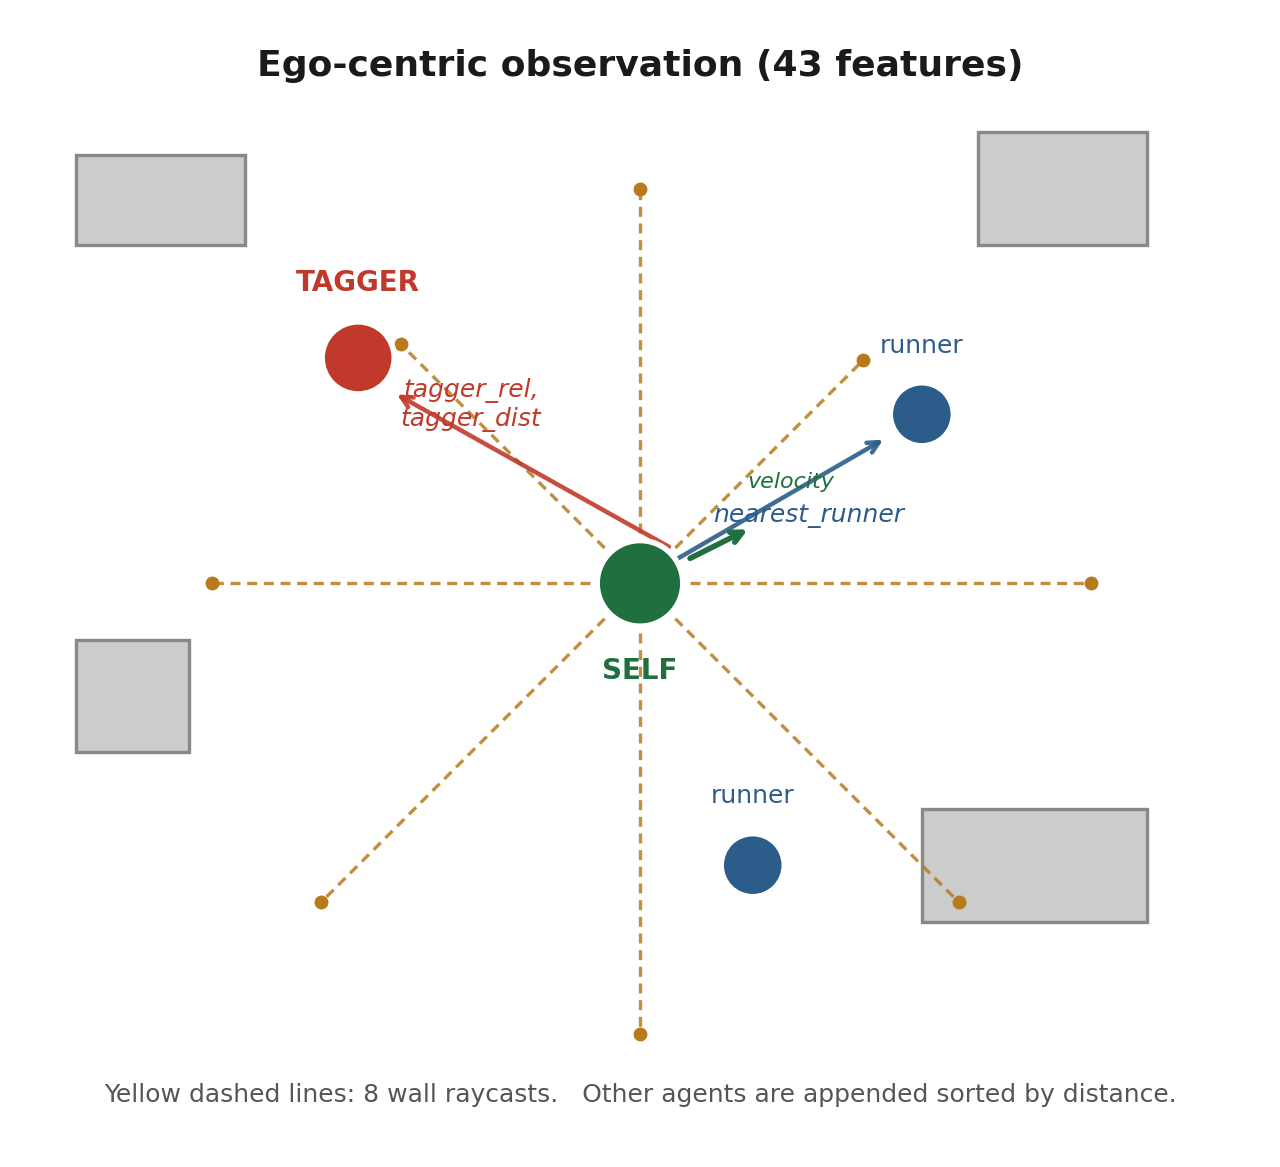
\includegraphics[width=0.95\columnwidth]{observation.png}}
\caption{Ego-centric observation. The agent (green) sits at the centre of its
view; eight wall raycasts return normalized distances, and the relative
positions and distances of the tagger (red), the nearest runner, and up to
six other agents are appended into a 43-dimensional vector.}
\label{fig:observation}
\end{figure}

\begin{table}[t]
\caption{Ego-Centric Observation (43 dimensions)}
\label{tab:obs}
\centering
\begin{tabular}{lcl}
\toprule
\textbf{Field} & \textbf{Dim} & \textbf{Description} \\
\midrule
self\_pos              & 2  & normalized $(x, y)$ position \\
self\_vel              & 2  & current velocity \\
is\_tagger             & 1  & role flag \\
tagger\_rel            & 2  & relative offset to tagger \\
tagger\_dist           & 1  & normalized distance to tagger \\
nearest\_runner\_rel   & 2  & relative offset to nearest runner \\
nearest\_runner\_dist  & 1  & normalized distance to nearest runner \\
wall\_rays             & 8  & 8-direction raycast distances \\
other\_agents          & 24 & up to 6 others $\times$ (rel\_pos, dist, role) \\
\bottomrule
\end{tabular}
\end{table}

\subsection{Reward Design (Plan C: Pure Proximity)}\label{sec:reward}

After iterating through several earlier reward designs (raw distance shaping,
distance-delta shaping, escalating time penalties), we converged on a
minimal \emph{pure proximity} scheme that satisfies three desiderata:
(i) terminal events dominate, so policies cannot gain by avoiding tag
events; (ii) shaping is symmetric across roles; and (iii) the gradient is
silent at long range so that the policy must learn navigation from the
observation rather than from the reward.

Let $d$ denote the Euclidean distance between two agents and let
$R = 140$~pixels (approximately 4.4 tiles). The proximity term is
\begin{equation}
\phi(d) = c \cdot \max\!\left(0,\; 1 - \frac{d}{R}\right)^{2},
\quad c = 0.27.
\label{eq:phi}
\end{equation}
This is quadratic, so the gradient is steepest near the tag zone where it
matters most, and identically zero outside the radius. The per-frame reward
is (with $i$ ranging over runners and $d_i$ the distance to runner $i$):
\begin{align}
r_{\text{tagger}} &=
    \begin{cases}
        +50 & \text{on tag,}\\
        -0.05 + \displaystyle\sum_{i} \phi(d_i) & \text{otherwise,}
    \end{cases}\\
r_{\text{runner}} &=
    \begin{cases}
        -80 & \text{on being tagged,}\\
        +0.10 - \phi(d_{\text{tagger}}) & \text{otherwise.}
    \end{cases}
\end{align}
The tag bonus and being-tagged penalty are intentionally asymmetric ($+50$
vs.\ $-80$) to push runners toward stronger caution than taggers' aggression.
Constant time pressure on the tagger ($-0.05$) and constant survival bonus
on the runner ($+0.10$) prevent both freezing and reward-farming.

\subsection{Dual-Role Architecture}\label{sec:dualrole}

\begin{figure}[t]
\centerline{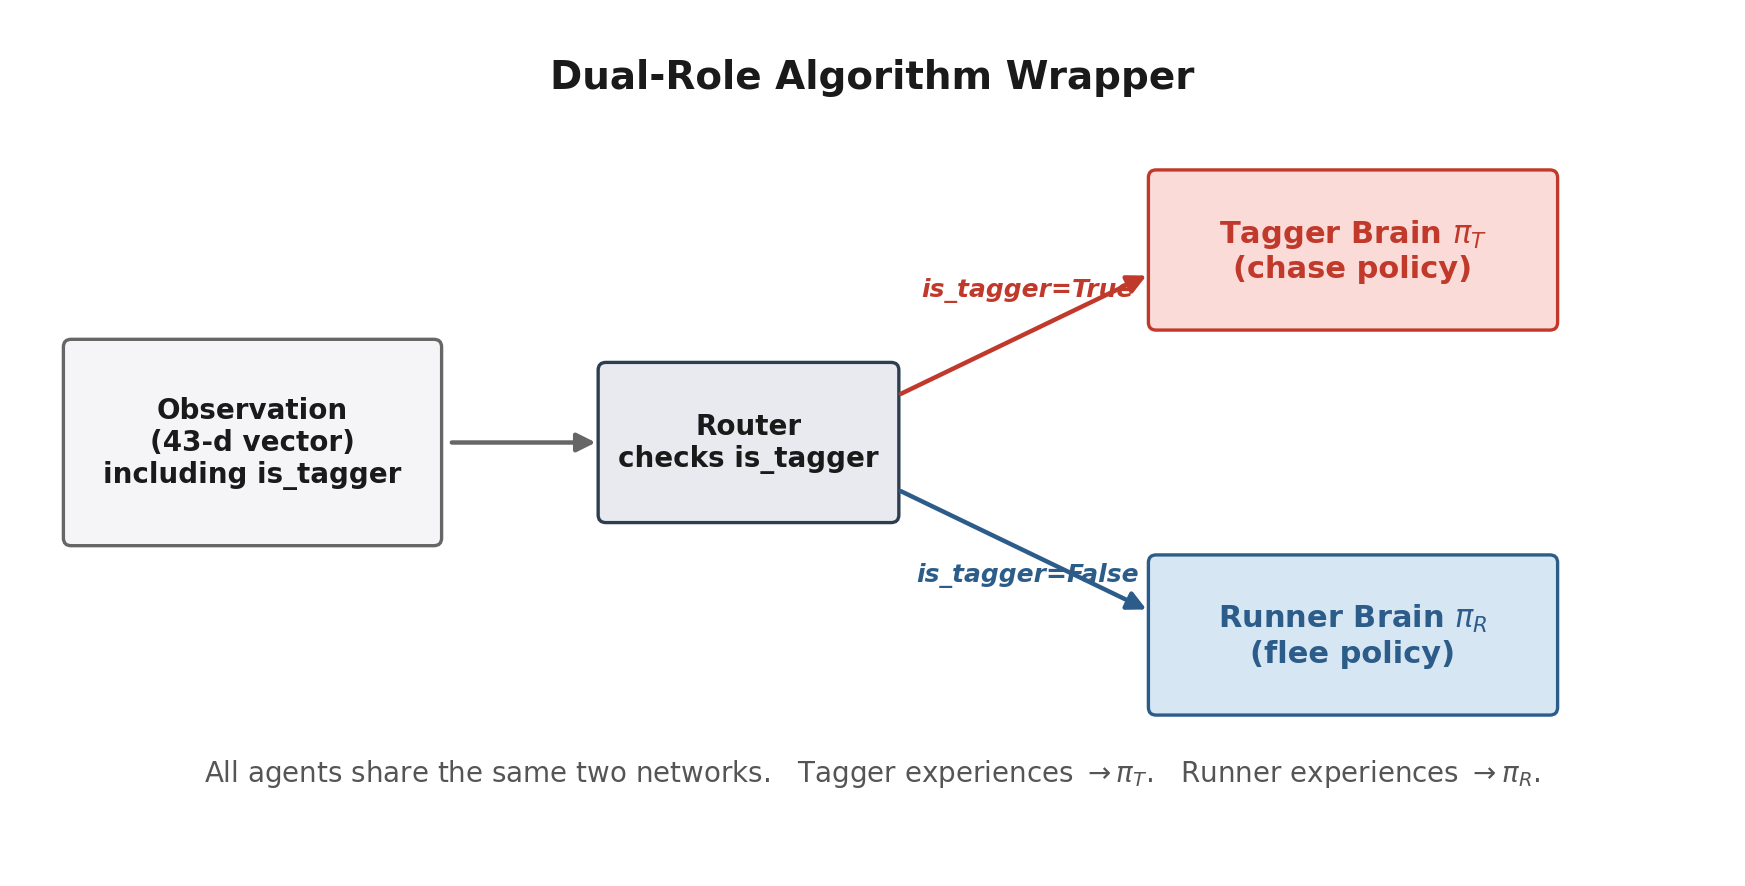
\includegraphics[width=0.95\columnwidth]{dual_role.png}}
\caption{Dual-role architecture. Each observation is routed by its
\texttt{is\_tagger} flag to one of two shared networks: a \emph{tagger
brain} ($\pi_T$) or a \emph{runner brain} ($\pi_R$). All six agents
contribute experience to the same two networks, so the role flip on a tag
event becomes a routing decision rather than a learning conflict.}
\label{fig:dualrole}
\end{figure}

Training a single network on both roles produces conflicting gradients:
the same observation can demand opposite actions depending on whether the
agent is the tagger or a runner, and the role flips abruptly during play.
We solve this with a wrapper class \texttt{DualRoleAlgorithm}
(Fig.~\ref{fig:dualrole}) that holds two underlying algorithm instances,
$\pi_T$ (tagger brain) and $\pi_R$ (runner brain). At each decision step the wrapper inspects
\texttt{observation["is\_tagger"]} and forwards the call to the appropriate
inner algorithm. Critically, all six agents in a simulation share the
\emph{same} two networks: tagger experiences from any agent contribute to
$\pi_T$, and runner experiences from any agent contribute to $\pi_R$. This
pools experience across the five concurrent runners while preserving
role-specific specialization, and resolves the conflicting-gradient problem
entirely. A side benefit is that $\pi_T$ and $\pi_R$ can be trained with
different algorithms (e.g., a Q-Learning tagger paired with a SARSA runner),
which we exploit for the simplified gridworld experiments.

\subsection{Algorithms}

All four algorithms inherit from \texttt{BaseRLAlgorithm} and implement
\texttt{select\_action(obs)}, \texttt{learn(s, a, r, s', done)}, and
save/load.

\textbf{Q-Learning} discretizes each continuous observation field into
between 4 and 9 bins, producing a hashable state key, and updates a Python
dictionary $Q\!:\!(s,a)\!\to\!\mathbb{R}$ with $\alpha=0.1$, $\gamma=0.95$,
and $\epsilon$-greedy exploration decaying from $1.0$ to $0.05$.

\textbf{SARSA} uses the same discretization but the on-policy update
$Q(s,a) \leftarrow Q(s,a) + \alpha\,(r + \gamma\,Q(s', a') - Q(s,a))$ where
$a'$ is the actual next action drawn from the policy.

\textbf{DQN} uses an MLP $Q_\theta(s, \cdot)$ that maps the 43-dimensional
observation to one Q-value per action, with experience replay (capacity
50k), a target network synchronized every 500 gradient steps, the Adam
optimizer ($\alpha=10^{-3}$), $\gamma=0.99$, and $\epsilon$ decaying linearly
from 1.0 to 0.05 over the first 50k steps. The loss is the Huber loss
between $Q_\theta(s,a)$ and $r + \gamma \max_{a'} Q_{\theta^-}(s', a')$.

\textbf{PPO} uses a shared-trunk actor--critic network with two hidden
layers (128 units, ReLU). Trajectories are collected for 256 environment
steps and then optimized with the clipped surrogate objective
($\epsilon=0.2$) for four epochs of mini-batch updates of size 64. We use
generalized advantage estimation ($\lambda=0.95$, $\gamma=0.99$), an entropy
bonus ($0.01$) to maintain exploration, and gradient clipping at norm 0.5.

\subsection{Training and Evaluation Pipeline}

A single script \texttt{run\_experiment.py} runs the entire workflow for any
algorithm. Training proceeds for a fixed number of epochs (each epoch is
2000 environment steps); two parallel headless simulations run in lock-step
and contribute experience to the shared dual-role networks. Checkpoints are
saved at epochs $\{2, 5, 10, 50, 100\}$ for shorter runs and additionally at
$\{200, 500, 1000\}$ for the long DQN run, plus a separate \emph{best-so-far}
checkpoint that captures the round with the highest tag count---important
for algorithms such as PPO that oscillate round-to-round.

Each saved checkpoint is then evaluated under three protocols
(Section~\ref{sec:eval-protocol}). During evaluation an algorithm-level
\texttt{eval\_mode} flag is set so that learn updates are disabled and the
policy is truly frozen. A fixed random seed across algorithms ensures fair
cross-checkpoint comparison. The pipeline finally produces learning curves,
per-epoch performance bars, role-trend line plots, role-diagnostic plots,
trajectory overlays, and 2D position heatmaps.

\subsection{Evaluation Protocols}\label{sec:eval-protocol}

We measure three quantities per checkpoint, each averaged over 20
evaluation episodes of 2000 steps:
\begin{itemize}
    \item \textbf{Joint evaluation:} both the tagger and runner brains are
    loaded; this measures the overall learned policy.
    \item \textbf{Isolated tagger evaluation:} the tagger brain is loaded
    but the runner brain is left untrained (random); higher tag counts
    indicate a stronger \emph{tagger}.
    \item \textbf{Isolated runner evaluation:} the runner brain is loaded
    but the tagger brain is random; \emph{lower} tag counts indicate
    stronger \emph{runners}.
\end{itemize}
We additionally export rendered MP4 videos for the joint and isolated evals
so that emergent movement patterns (corner-camping, wall-hugging escape,
direct interception) can be qualitatively recognized.

\subsection{Human-in-the-Loop Mode}

Beyond the headless training and evaluation pipeline, the environment
supports a \emph{human-in-the-loop} game mode in which a human player
controls one entity with the keyboard while the remaining agents continue to
learn online. This mode is useful both as a sanity check (a fresh-trained
policy that consistently dodges or catches a human player is a strong
qualitative signal) and as a means of testing robustness to non-Markovian,
intent-driven behavior the agent never saw in self-play.

\section{Results and Analysis}\label{sec:results}

\subsection{Experimental Setup}

All experiments use the default \texttt{level\_small} map and the
pure-proximity reward of Section~\ref{sec:reward}. Training and evaluation
share identical observation, reward, action space, and decision interval to
ensure that any cross-algorithm differences arise from the algorithm itself
rather than from environment differences. All experiments run on
CPU---PyTorch's MPS backend was found to be incompatible with our
small-tensor workload, and CPU training is more than fast enough at the
network sizes used here ($\sim$37k PPO parameters).

\subsection{Tabular Methods Fail on the Full Game}

\begin{figure*}[t]
\centerline{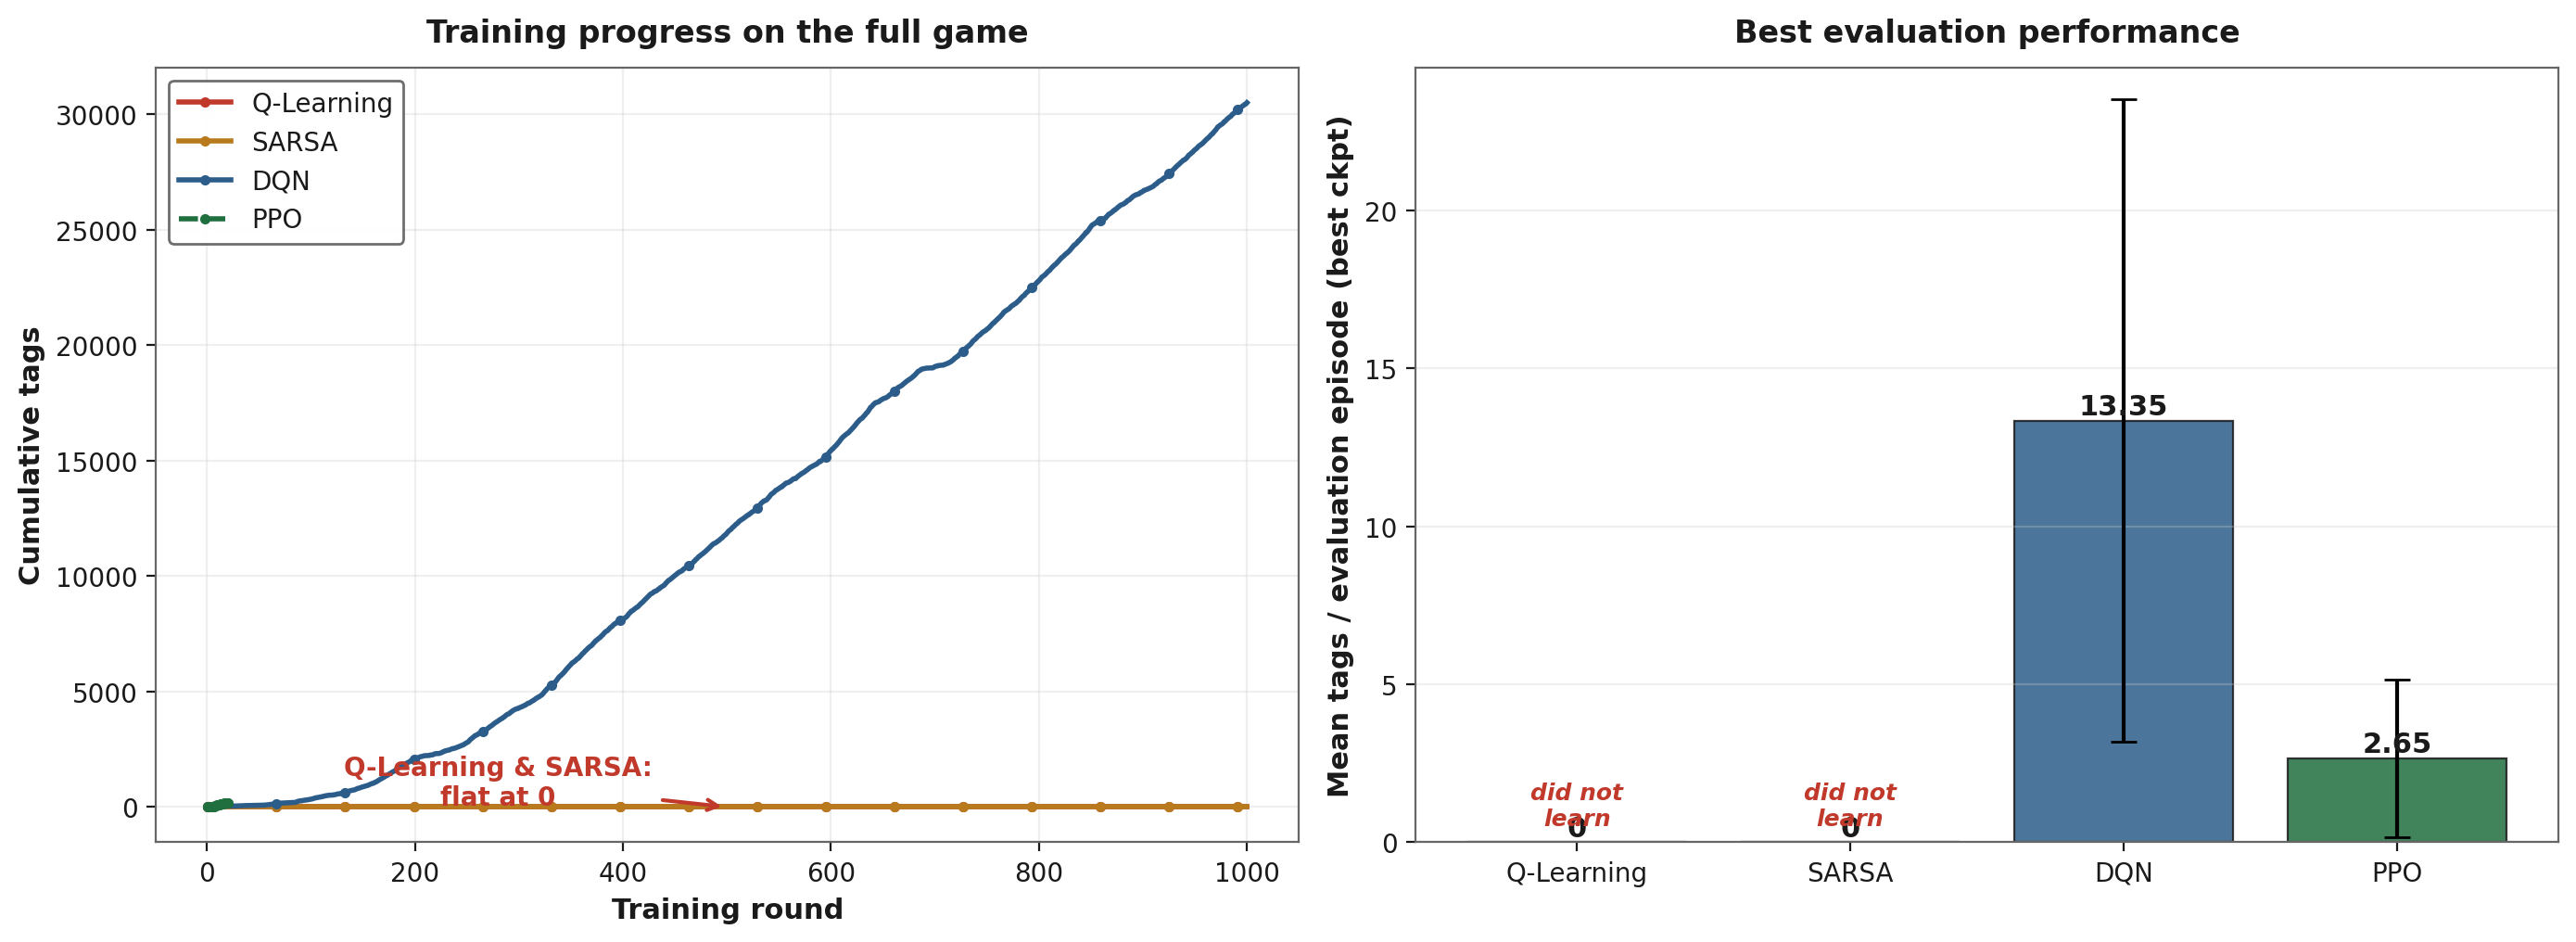
\includegraphics[width=0.92\textwidth]{tabular_failure.png}}
\caption{Algorithm comparison on the full Tag environment.
\textbf{Left:} cumulative tags over training rounds. Q-Learning (red) and
SARSA (orange) remain flat at zero across all 1000 rounds, while DQN (blue)
and PPO (green) accumulate tags steadily. \textbf{Right:} best
joint-evaluation tag count per algorithm. The two tabular methods score
exactly zero, while DQN reaches a peak of 13.35 mean tags per evaluation
episode.}
\label{fig:tabular-failure}
\end{figure*}

We trained Q-Learning and SARSA on the full Tag environment for 1000 epochs
each, with checkpoints at $\{10, 50, 100, 200, 500, 1000\}$ and 20
evaluation episodes per checkpoint. Both algorithms produced
\textbf{zero successful tags at every checkpoint}
(Fig.~\ref{fig:tabular-failure})---a complete failure to learn. The cause is a combination of three factors:
(i) even after binning each of the 43 observation fields, the discretized
state space contains many millions of cells, most of which are visited at
most once during 1000 epochs; (ii) the game has no clean episode boundary
(it runs forever), so there is no $\mathit{done}$ signal that meaningfully
terminates the Bellman recursion; and (iii) Q-tables cannot generalize
across similar-but-distinct states.

\subsection{Simplified Gridworld Recovers Tabular Performance}

To verify that the failure was structural rather than implementation
related, we built a simplified $10\times 10$ turn-based gridworld with one
tagger and one runner. The state space is exactly $10^4$ cells---tractable
for a Q-table. We trained Q-Learning and SARSA in three phases:
(1) tagger trained against a random runner; (2) runner trained against the
frozen trained tagger; (3) trained tagger vs.\ trained runner for
evaluation. Both algorithms converged within a few thousand episodes.
Consistent with the classical Cliff-Walking analogue, we observed that
Q-Learning produced more aggressive direct-pursuit taggers, while SARSA
produced safer wall-hugging runners.

\subsection{Joint Evaluation on the Full Game}

PPO and DQN were trained on the full Tag environment with two parallel
simulations contributing experience to the shared dual-role networks. PPO
was evaluated at epoch 20 only (a short pilot run constrained by training
time). DQN was trained in two configurations---an early run (\texttt{dqn/},
100 epochs) with weaker hyperparameters, and a refined run
(\texttt{dqn3.0/}, 1000 epochs) which is the basis of the main results.

Table~\ref{tab:joint} summarizes the best joint-evaluation tag counts for
each algorithm; Fig.~\ref{fig:dqn-curve} shows the DQN (v3.0) training
curve over the full 1000-epoch run. PPO reached 2.65 tags per episode at
its only evaluated checkpoint; the refined DQN run reached a peak of 13.35
tags at epoch 500 and a best-checkpoint score of 10.7 tags. Tabular methods
scored zero throughout.

\begin{figure}[t]
\centerline{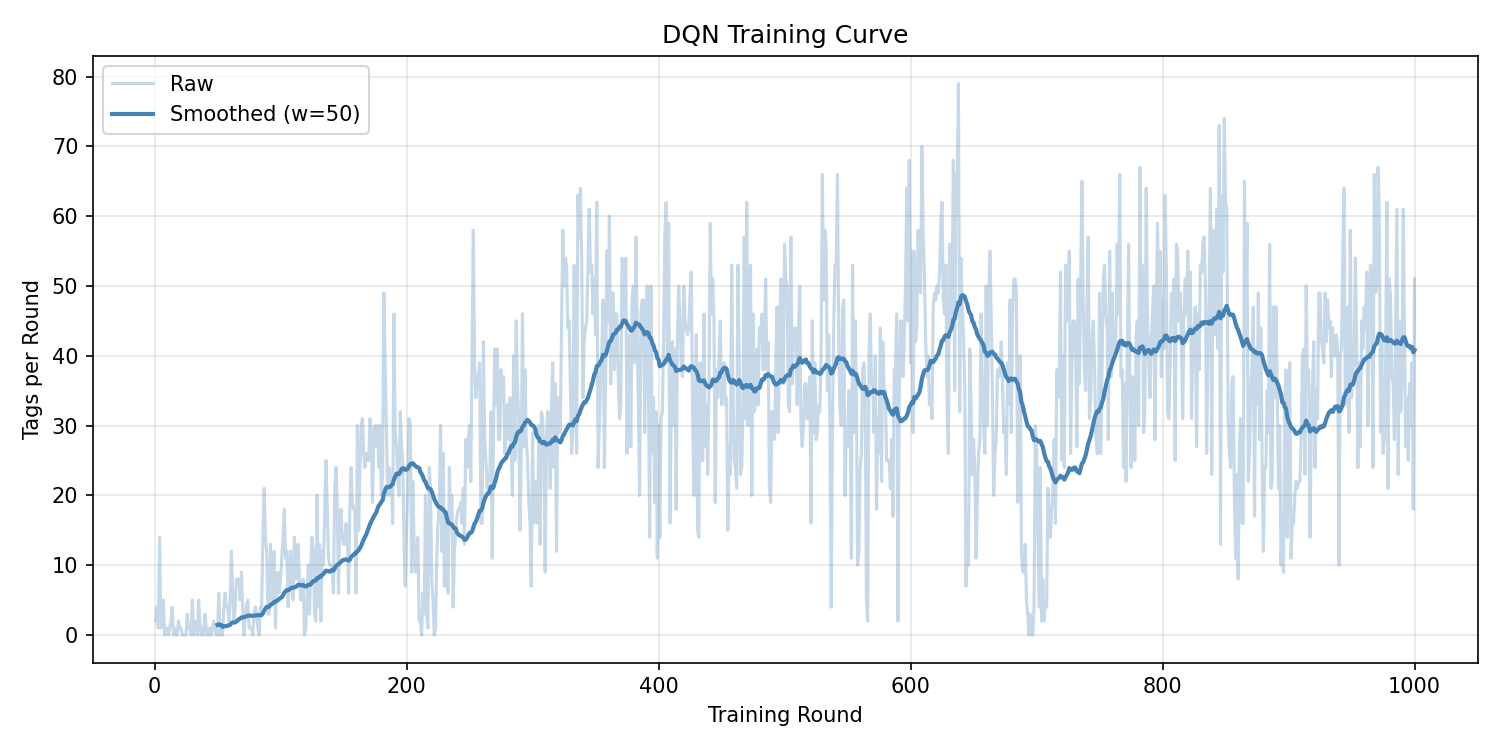
\includegraphics[width=0.95\columnwidth]{dqn_training_curve.png}}
\caption{DQN (v3.0) training curve over 1000 epochs. The blue line is the
raw per-round tag count; the smoothed curve shows the rising trend.
Performance climbs sharply between epochs 100 and 500, then plateaus and
oscillates around a high mean.}
\label{fig:dqn-curve}
\end{figure}

\begin{table}[t]
\caption{Best Joint Evaluation (Mean Tags per 2000-Step Episode)}
\label{tab:joint}
\centering
\begin{tabular}{lccc}
\toprule
\textbf{Algorithm} & \textbf{Best epoch} & \textbf{Mean tags} & \textbf{Std} \\
\midrule
Q-Learning  & any              & 0.00  & 0.00 \\
SARSA       & any              & 0.00  & 0.00 \\
PPO         & 20               & 2.65  & 2.50 \\
DQN (v1)    & 50               & 0.85  & 1.53 \\
DQN (v3.0)  & 500              & \textbf{13.35} & 10.18 \\
DQN (v3.0, best ckpt) & ---    & 10.70 & 6.16 \\
\bottomrule
\end{tabular}
\end{table}

\subsection{Isolated Role Evaluation Reveals an Asymmetry}

Joint scores conflate tagger and runner skill. The isolated protocol
(Section~\ref{sec:eval-protocol}) disentangles them.
Table~\ref{tab:role} and Fig.~\ref{fig:role-eval} report the DQN (v3.0)
results across training. Two clear patterns emerge.

\begin{figure}[t]
\centerline{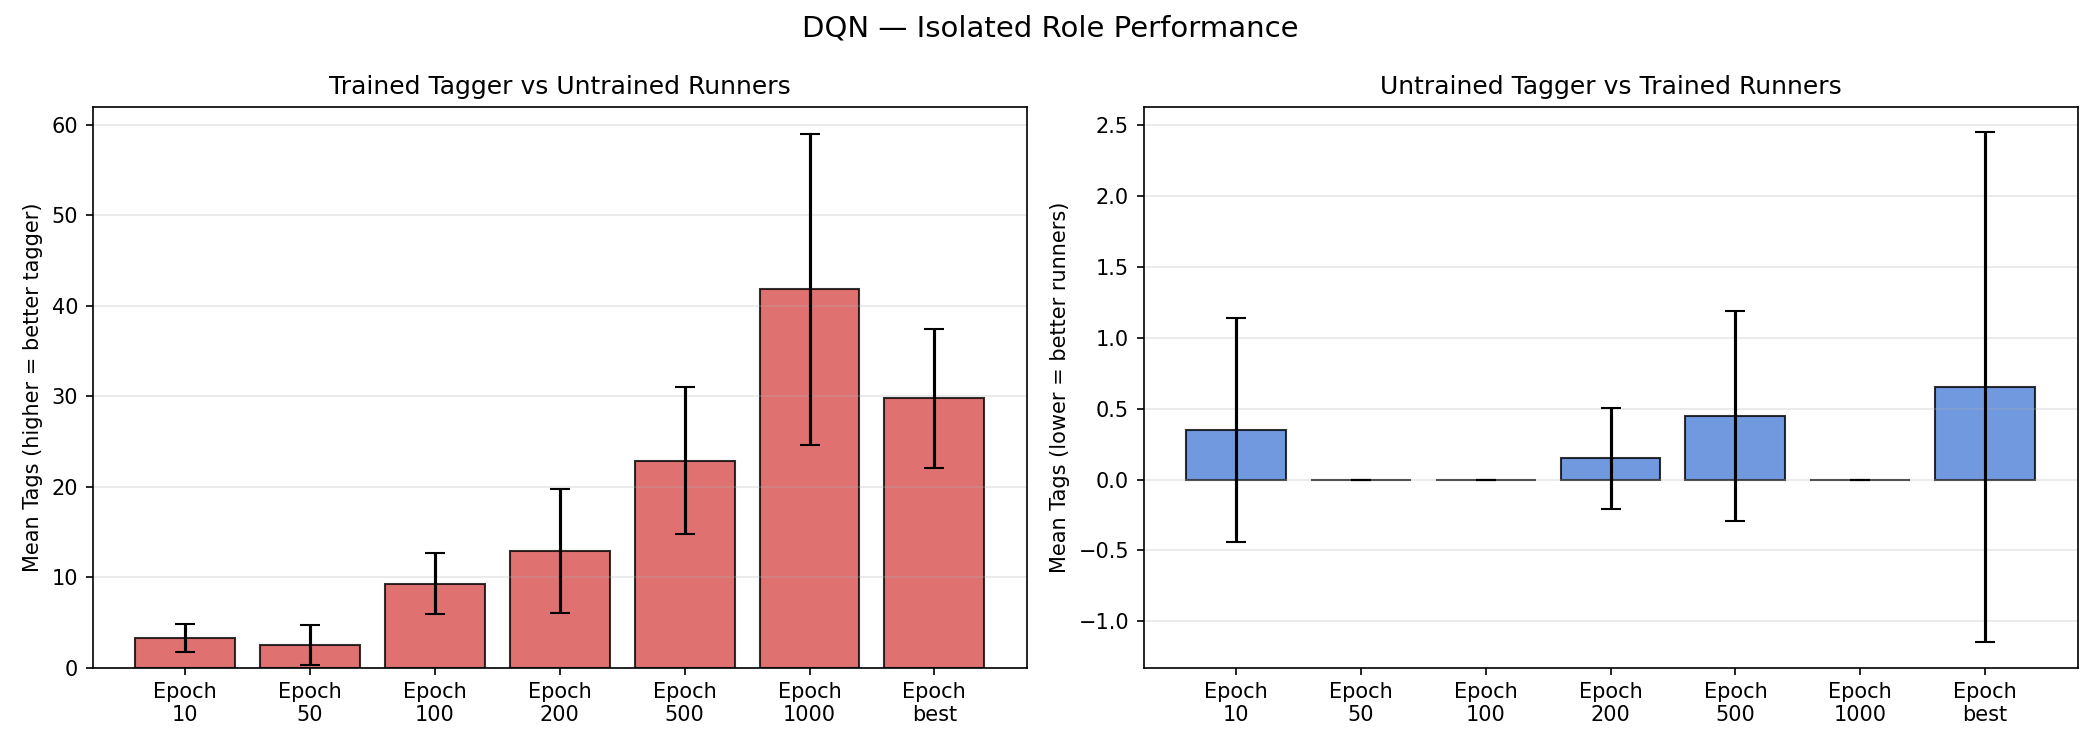
\includegraphics[width=0.95\columnwidth]{dqn_role_evaluation.png}}
\caption{Isolated role evaluation for DQN (v3.0). Left: trained tagger vs.
random runners (higher is better tagger). Right: trained runners vs.\
random tagger (lower is better runner). The tagger improves monotonically
from 3.3 to 41.85 tags per episode; the runner remains strong throughout
($\le 0.65$).}
\label{fig:role-eval}
\end{figure}

\begin{table}[t]
\caption{Isolated Role Evaluation -- DQN (v3.0)}
\label{tab:role}
\centering
\begin{tabular}{lcc}
\toprule
\textbf{Epoch} & \textbf{Tagger tags} $\uparrow$ & \textbf{Runner tags} $\downarrow$ \\
\midrule
10   & 3.30  $\pm$ 1.52  & 0.35 $\pm$ 0.79 \\
50   & 2.50  $\pm$ 2.18  & 0.00 $\pm$ 0.00 \\
100  & 9.25  $\pm$ 3.37  & 0.00 $\pm$ 0.00 \\
200  & 12.90 $\pm$ 6.87  & 0.15 $\pm$ 0.36 \\
500  & 22.90 $\pm$ 8.16  & 0.45 $\pm$ 0.74 \\
1000 & \textbf{41.85 $\pm$ 17.19} & 0.00 $\pm$ 0.00 \\
best & 29.80 $\pm$ 7.67  & 0.65 $\pm$ 1.80 \\
\bottomrule
\end{tabular}
\end{table}

First, the tagger brain improves \emph{monotonically} with training,
climbing from 3.3 tags at epoch 10 to 41.85 tags at epoch 1000 against a
random opponent---a more than $12\times$ improvement. Second, the runner
brain remains essentially flat at $0$--$0.65$ tags throughout: a random
tagger almost never catches the trained runners. This is excellent runner
performance in absolute terms, but it reflects the difficulty of the runner
problem more than rapid learning, since a random tagger is itself extremely
weak.

The asymmetry has two implications. (i) The dual-role architecture
successfully decouples the two roles---runners do not catastrophically
forget their flee policy as the tagger improves, and vice versa.
(ii) Joint evaluation alone would have hidden this asymmetry: the joint
score peaks near epoch 500 and dips slightly at 1000, but the isolated
tagger continues to improve dramatically. The dip at 1000 is therefore
explained by runners catching up rather than by tagger regression.

\subsection{Behavioral Observations}

We exported rendered evaluation videos for each checkpoint to qualitatively
recognize the moving patterns of each role. Trained taggers consistently
exhibit \emph{direct interception}, anticipating the runner's heading
rather than chasing the runner's current position---an emergent behavior
never explicitly rewarded. Runners learn to \emph{wall-hug} when the tagger
is far and to \emph{break perpendicular} to the tagger's pursuit vector
when close. We also observed pathological patterns at low epochs:
corner-camping by runners (high reward at the cost of immobility) and
stand-still equilibria when both agents have weakly initialized Q-values.
The pure-proximity reward of Section~\ref{sec:reward} eliminates
corner-camping by making the danger penalty escalate quadratically near the
tagger, forcing motion. Fig.~\ref{fig:trajectory} overlays the agent
trajectories from a single evaluation episode of the best DQN checkpoint;
runners trace clear arcs along the room perimeter while the tagger
converges on intercept points rather than chasing through the centre.

\begin{figure}[t]
\centerline{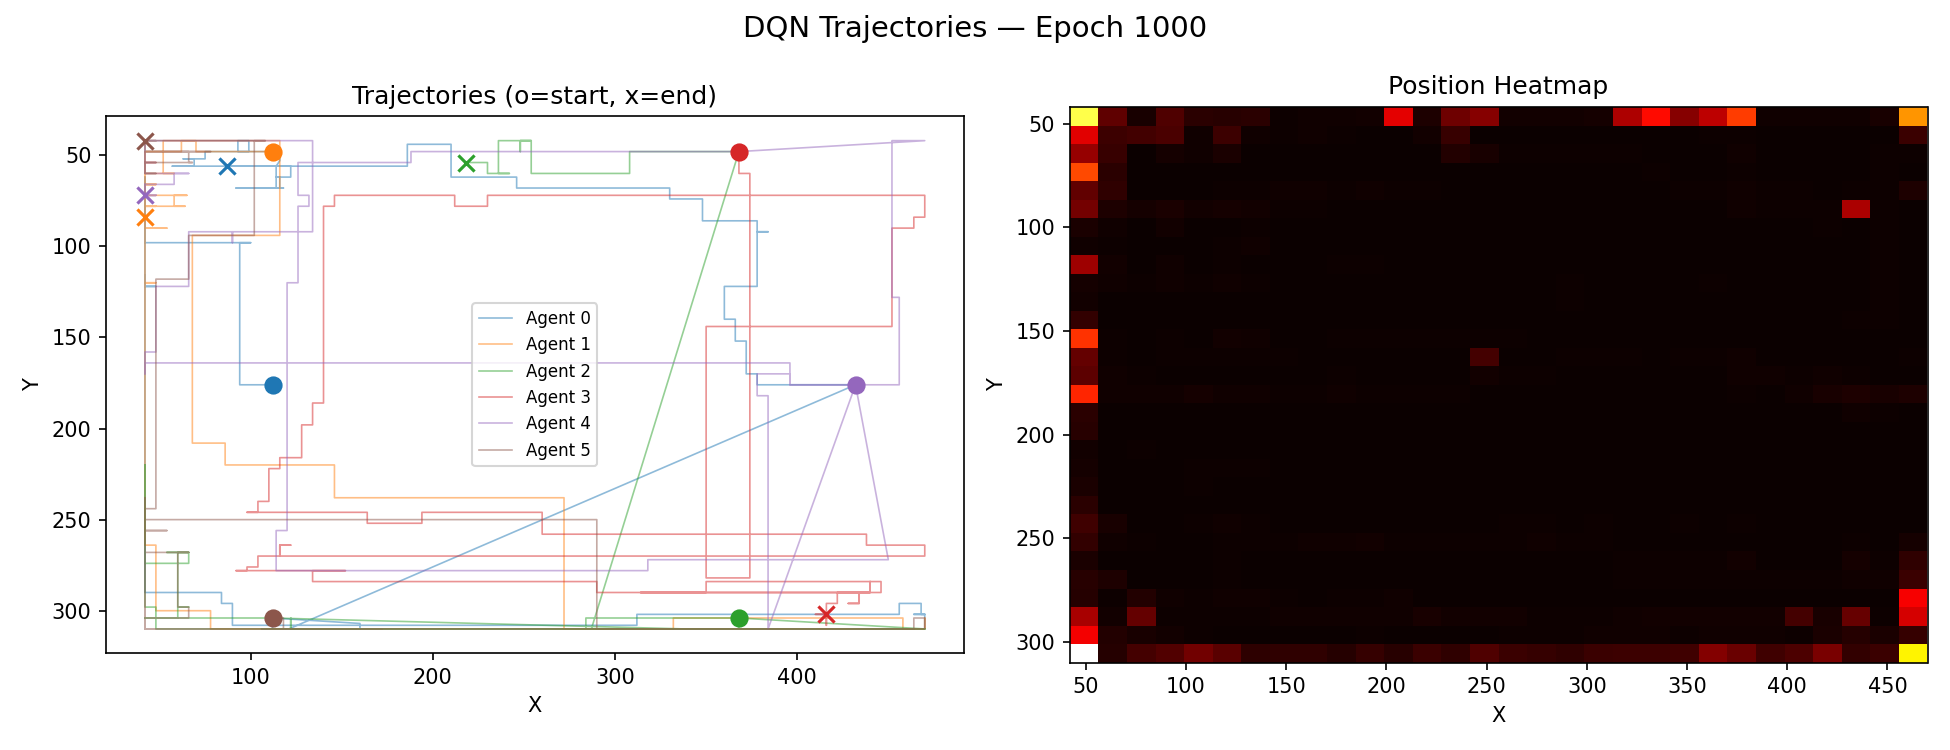
\includegraphics[width=0.95\columnwidth]{dqn_trajectory_1000.png}}
\caption{Agent trajectories from a single evaluation episode of the best
DQN (v3.0) checkpoint. Each colour is one agent. Runners (blue/green
tones) trace perimeter arcs; the tagger's path (red) shows direct
interception rather than tail-chasing.}
\label{fig:trajectory}
\end{figure}

\subsection{Discussion}\label{sec:results-discussion}

\textbf{Why tabular methods fail and deep methods succeed.} The contrast
between tabular failure on the full game and tabular success on the
simplified gridworld is the single clearest result of this study. Tabular
methods need a finite, hashable, and \emph{coverable} state space, which the
full continuous environment does not provide. Deep methods generalize across
nearby states via function approximation, so a never-seen state is not
catastrophic. The lesson is that algorithm choice is dictated by problem
structure as much as by algorithm sophistication.

\textbf{Q-Learning vs.\ SARSA in the gridworld.} The gridworld results
reproduce the classical Cliff-Walking-style asymmetry. Q-Learning's
off-policy update is optimistic (it bootstraps from
$\max_{a'} Q(s', a')$ rather than the actual next action) and produces
aggressive direct-pursuit taggers that close distance even when an
exploratory move would briefly increase risk. SARSA's on-policy update is
conservative (it bootstraps from the actual next action, including
$\epsilon$-random ones) and produces runners that maintain a safety buffer
against their own random exploration. The dual-role architecture exposed
this difference cleanly because each role can be trained with a different
algorithm if desired.

\textbf{Limitations.} (i) PPO was only evaluated at a short 20-epoch pilot;
a longer PPO run is necessary for a fair head-to-head against the 1000-epoch
DQN. (ii) Our simplified gridworld results, while qualitatively striking,
are based on a small number of seeds and would benefit from statistical
hypothesis testing. (iii) The \texttt{level\_small} map's scale and density
were tuned for fast iteration, not for representative complexity; behavior
on \texttt{level\_01} (the larger map) is left for future work.

\section{Conclusion and Future Work}\label{sec:conclusion}

We presented \textit{Learn To Tag}, a multi-agent Tag environment as a
controlled testbed for benchmarking RL algorithms under mid-episode role
switching. The \emph{dual-role} architecture---two shared networks routed at
runtime by the agent's role flag---resolves the conflicting-gradient problem
of single-network training and pools experience across concurrent runners.
The \emph{pure-proximity} reward eliminates several pathological behaviors
(corner-camping, freezing) while keeping the gradient silent at long range
so the policy must learn to navigate from observation. The
\emph{isolated role evaluation} protocol exposes asymmetric skill
development between the two brains that joint evaluation hides.

Empirically, tabular Q-Learning and SARSA fail completely on the full
continuous environment but succeed cleanly on a simplified turn-based
gridworld variant, reproducing the Cliff-Walking risk-profile contrast.
DQN trained for 1000 epochs reaches an isolated-tagger score of 41.85 tags
per evaluation episode and a best-checkpoint joint score of 10.7 tags;
PPO at a short pilot reaches 2.65 joint tags. Across all deep runs the
tagger brain develops faster than the runner brain, a finding that joint
evaluation alone would obscure.

\textbf{Future work.} Several extensions are immediate.
(i) Mixing algorithms across roles---e.g., a Q-Learning tagger paired with
a SARSA runner---to exploit each algorithm's risk profile.
(ii) Cooperative runner behavior using multi-agent policy gradient methods.
(iii) Curriculum learning across the small, medium, and large maps,
transferring weights between phases.
(iv) Function approximation versions of Q-Learning and SARSA (linear or
tile coding) to bridge the tabular--deep gap on the full environment.
(v) A larger-scale human-in-the-loop study to characterize how trained
policies generalize to real human players.

\section*{Acknowledgment}

We thank the course instructors and teaching assistants for guidance, and
the open-source Pygame and PyTorch communities whose tools made this work
practical.

\begin{thebibliography}{00}
\bibitem{watkins1989} C.~J.~C.~H.~Watkins, ``Learning from Delayed Rewards,'' Ph.D. dissertation, Cambridge University, 1989.
\bibitem{rummery1994} G.~A.~Rummery and M.~Niranjan, ``On-line Q-learning using connectionist systems,'' Cambridge University Engineering Dept., Tech. Rep. CUED/F-INFENG/TR 166, 1994.
\bibitem{sutton2018} R.~S.~Sutton and A.~G.~Barto, \emph{Reinforcement Learning: An Introduction}, 2nd ed.\ \ \ Cambridge, MA: MIT Press, 2018.
\bibitem{mnih2015} V.~Mnih \emph{et al.}, ``Human-level control through deep reinforcement learning,'' \emph{Nature}, vol.~518, no.~7540, pp.~529--533, 2015.
\bibitem{vanhasselt2016} H.~van~Hasselt, A.~Guez, and D.~Silver, ``Deep reinforcement learning with double Q-learning,'' in \emph{Proc.\ AAAI}, 2016.
\bibitem{schulman2017} J.~Schulman, F.~Wolski, P.~Dhariwal, A.~Radford, and O.~Klimov, ``Proximal policy optimization algorithms,'' \emph{arXiv preprint arXiv:1707.06347}, 2017.
\bibitem{yu2022} C.~Yu \emph{et al.}, ``The Surprising Effectiveness of PPO in Cooperative Multi-Agent Games,'' in \emph{Proc.\ NeurIPS Datasets and Benchmarks}, 2022.
\bibitem{baker2020} B.~Baker \emph{et al.}, ``Emergent Tool Use From Multi-Agent Autocurricula,'' in \emph{Proc.\ ICLR}, 2020.
\bibitem{schaul2015} T.~Schaul, D.~Horgan, K.~Gregor, and D.~Silver, ``Universal value function approximators,'' in \emph{Proc.\ ICML}, 2015.
\bibitem{andreas2017} J.~Andreas, D.~Klein, and S.~Levine, ``Modular multitask reinforcement learning with policy sketches,'' in \emph{Proc.\ ICML}, 2017.
\end{thebibliography}

\end{document}
